\documentclass[twoside]{book}

% Packages required by doxygen
\usepackage{calc}
\usepackage{doxygen}
\usepackage{graphicx}
\usepackage[utf8]{inputenc}
\usepackage{makeidx}
\usepackage{multicol}
\usepackage{multirow}
\usepackage{textcomp}
\usepackage[table]{xcolor}

% Font selection
\usepackage[T1]{fontenc}
\usepackage{mathptmx}
\usepackage[scaled=.90]{helvet}
\usepackage{courier}
\usepackage{amssymb}
\usepackage{sectsty}
\renewcommand{\familydefault}{\sfdefault}
\allsectionsfont{%
  \fontseries{bc}\selectfont%
  \color{darkgray}%
}
\renewcommand{\DoxyLabelFont}{%
  \fontseries{bc}\selectfont%
  \color{darkgray}%
}

% Page & text layout
\usepackage{geometry}
\geometry{%
  a4paper,%
  top=2.5cm,%
  bottom=2.5cm,%
  left=2.5cm,%
  right=2.5cm%
}
\tolerance=750
\hfuzz=15pt
\hbadness=750
\setlength{\emergencystretch}{15pt}
\setlength{\parindent}{0cm}
\setlength{\parskip}{0.2cm}
\makeatletter
\renewcommand{\paragraph}{%
  \@startsection{paragraph}{4}{0ex}{-1.0ex}{1.0ex}{%
    \normalfont\normalsize\bfseries\SS@parafont%
  }%
}
\renewcommand{\subparagraph}{%
  \@startsection{subparagraph}{5}{0ex}{-1.0ex}{1.0ex}{%
    \normalfont\normalsize\bfseries\SS@subparafont%
  }%
}
\makeatother

% Headers & footers
\usepackage{fancyhdr}
\pagestyle{fancyplain}
\fancyhead[LE]{\fancyplain{}{\bfseries\thepage}}
\fancyhead[CE]{\fancyplain{}{}}
\fancyhead[RE]{\fancyplain{}{\bfseries\leftmark}}
\fancyhead[LO]{\fancyplain{}{\bfseries\rightmark}}
\fancyhead[CO]{\fancyplain{}{}}
\fancyhead[RO]{\fancyplain{}{\bfseries\thepage}}
\fancyfoot[LE]{\fancyplain{}{}}
\fancyfoot[CE]{\fancyplain{}{}}
\fancyfoot[RE]{\fancyplain{}{\bfseries\scriptsize Generated on Tue Jun 23 2015 18\-:12\-:42 for H\-O\-P3\-D by Doxygen }}
\fancyfoot[LO]{\fancyplain{}{\bfseries\scriptsize Generated on Tue Jun 23 2015 18\-:12\-:42 for H\-O\-P3\-D by Doxygen }}
\fancyfoot[CO]{\fancyplain{}{}}
\fancyfoot[RO]{\fancyplain{}{}}
\renewcommand{\footrulewidth}{0.4pt}
\renewcommand{\chaptermark}[1]{%
  \markboth{#1}{}%
}
\renewcommand{\sectionmark}[1]{%
  \markright{\thesection\ #1}%
}

% Indices & bibliography
\usepackage{natbib}
\usepackage[titles]{tocloft}
\setcounter{tocdepth}{3}
\setcounter{secnumdepth}{5}
\makeindex

% Hyperlinks (required, but should be loaded last)
\usepackage{ifpdf}
\ifpdf
  \usepackage[pdftex,pagebackref=true]{hyperref}
\else
  \usepackage[ps2pdf,pagebackref=true]{hyperref}
\fi
\hypersetup{%
  colorlinks=true,%
  linkcolor=blue,%
  citecolor=blue,%
  unicode%
}

% Custom commands
\newcommand{\clearemptydoublepage}{%
  \newpage{\pagestyle{empty}\cleardoublepage}%
}


%===== C O N T E N T S =====

\begin{document}

% Titlepage & ToC
\hypersetup{pageanchor=false}
\pagenumbering{roman}
\begin{titlepage}
\vspace*{7cm}
\begin{center}%
{\Large H\-O\-P3\-D }\\
\vspace*{1cm}
{\large Generated by Doxygen 1.8.6}\\
\vspace*{0.5cm}
{\small Tue Jun 23 2015 18:12:42}\\
\end{center}
\end{titlepage}
\clearemptydoublepage
\tableofcontents
\clearemptydoublepage
\pagenumbering{arabic}
\hypersetup{pageanchor=true}

%--- Begin generated contents ---
\chapter{Namespace Index}
\section{Namespace List}
Here is a list of all namespaces with brief descriptions\-:\begin{DoxyCompactList}
\item\contentsline{section}{\hyperlink{namespacehop3d}{hop3d} }{\pageref{namespacehop3d}}{}
\end{DoxyCompactList}

\chapter{Hierarchical Index}
\section{Class Hierarchy}
This inheritance list is sorted roughly, but not completely, alphabetically\-:\begin{DoxyCompactList}
\item \contentsline{section}{Cloud}{\pageref{class_cloud}}{}
\begin{DoxyCompactList}
\item \contentsline{section}{Part\-Cloud}{\pageref{class_part_cloud}}{}
\item \contentsline{section}{Point\-Cloud}{\pageref{class_point_cloud}}{}
\end{DoxyCompactList}
\item \contentsline{section}{Graph\-Builder}{\pageref{class_graph_builder}}{}
\item \contentsline{section}{Layer\-Filterer}{\pageref{class_layer_filterer}}{}
\item \contentsline{section}{Layer\-Vocabulary}{\pageref{class_layer_vocabulary}}{}
\item \contentsline{section}{Local\-Inhibiter}{\pageref{class_local_inhibiter}}{}
\item \contentsline{section}{Object\-Graph}{\pageref{class_object_graph}}{}
\item \contentsline{section}{Part}{\pageref{class_part}}{}
\begin{DoxyCompactList}
\item \contentsline{section}{Part\-Realization}{\pageref{class_part_realization}}{}
\end{DoxyCompactList}
\item \contentsline{section}{Part\-Selector}{\pageref{class_part_selector}}{}
\item \contentsline{section}{Reader}{\pageref{class_reader}}{}
\item \contentsline{section}{Statistics\-Builder}{\pageref{class_statistics_builder}}{}
\item \contentsline{section}{Vocabulary}{\pageref{class_vocabulary}}{}
\item \contentsline{section}{Writer}{\pageref{class_writer}}{}
\end{DoxyCompactList}

\chapter{Class Index}
\section{Class List}
Here are the classes, structs, unions and interfaces with brief descriptions\-:\begin{DoxyCompactList}
\item\contentsline{section}{\hyperlink{class_cloud}{Cloud} }{\pageref{class_cloud}}{}
\item\contentsline{section}{\hyperlink{class_graph_builder}{Graph\-Builder} }{\pageref{class_graph_builder}}{}
\item\contentsline{section}{\hyperlink{class_layer_filterer}{Layer\-Filterer} }{\pageref{class_layer_filterer}}{}
\item\contentsline{section}{\hyperlink{class_layer_vocabulary}{Layer\-Vocabulary} }{\pageref{class_layer_vocabulary}}{}
\item\contentsline{section}{\hyperlink{class_local_inhibiter}{Local\-Inhibiter} }{\pageref{class_local_inhibiter}}{}
\item\contentsline{section}{\hyperlink{class_object_graph}{Object\-Graph} }{\pageref{class_object_graph}}{}
\item\contentsline{section}{\hyperlink{class_part}{Part} }{\pageref{class_part}}{}
\item\contentsline{section}{\hyperlink{class_part_cloud}{Part\-Cloud} }{\pageref{class_part_cloud}}{}
\item\contentsline{section}{\hyperlink{class_part_realization}{Part\-Realization} }{\pageref{class_part_realization}}{}
\item\contentsline{section}{\hyperlink{class_part_selector}{Part\-Selector} }{\pageref{class_part_selector}}{}
\item\contentsline{section}{\hyperlink{class_point_cloud}{Point\-Cloud} }{\pageref{class_point_cloud}}{}
\item\contentsline{section}{\hyperlink{class_reader}{Reader} }{\pageref{class_reader}}{}
\item\contentsline{section}{\hyperlink{class_statistics_builder}{Statistics\-Builder} }{\pageref{class_statistics_builder}}{}
\item\contentsline{section}{\hyperlink{class_vocabulary}{Vocabulary} }{\pageref{class_vocabulary}}{}
\item\contentsline{section}{\hyperlink{class_writer}{Writer} }{\pageref{class_writer}}{}
\end{DoxyCompactList}

\chapter{File Index}
\section{File List}
Here is a list of all files with brief descriptions\-:\begin{DoxyCompactList}
\item\contentsline{section}{\hyperlink{main_8cpp}{main.\-cpp} }{\pageref{main_8cpp}}{}
\item\contentsline{section}{include/\-Apps/\-Inference/\hyperlink{_inference_2_data_8h}{Data.\-h} }{\pageref{_inference_2_data_8h}}{}
\item\contentsline{section}{include/\-Apps/\-Inference/\hyperlink{_inference_8h}{Inference.\-h} }{\pageref{_inference_8h}}{}
\item\contentsline{section}{include/\-Apps/\-Learning/\hyperlink{_learning_2_data_8h}{Data.\-h} }{\pageref{_learning_2_data_8h}}{}
\item\contentsline{section}{include/\-Apps/\-Learning/\hyperlink{_learning_8h}{Learning.\-h} }{\pageref{_learning_8h}}{}
\item\contentsline{section}{include/\-Core/\hyperlink{_graph_builder_8h}{Graph\-Builder.\-h} }{\pageref{_graph_builder_8h}}{}
\item\contentsline{section}{include/\-Core/\hyperlink{_layer_filterer_8h}{Layer\-Filterer.\-h} }{\pageref{_layer_filterer_8h}}{}
\item\contentsline{section}{include/\-Core/\hyperlink{_local_inhibiter_8h}{Local\-Inhibiter.\-h} }{\pageref{_local_inhibiter_8h}}{}
\item\contentsline{section}{include/\-Core/\hyperlink{_part_selector_8h}{Part\-Selector.\-h} }{\pageref{_part_selector_8h}}{}
\item\contentsline{section}{include/\-Core/\hyperlink{_statistics_builder_8h}{Statistics\-Builder.\-h} }{\pageref{_statistics_builder_8h}}{}
\item\contentsline{section}{include/\-Data/\hyperlink{_cloud_8h}{Cloud.\-h} }{\pageref{_cloud_8h}}{}
\item\contentsline{section}{include/\-Data/\hyperlink{_defs_8h}{Defs.\-h} }{\pageref{_defs_8h}}{}
\item\contentsline{section}{include/\-Data/\hyperlink{_graph_8h}{Graph.\-h} }{\pageref{_graph_8h}}{}
\item\contentsline{section}{include/\-Data/\hyperlink{_part_8h}{Part.\-h} }{\pageref{_part_8h}}{}
\item\contentsline{section}{include/\-Data/\hyperlink{_vocabulary_8h}{Vocabulary.\-h} }{\pageref{_vocabulary_8h}}{}
\item\contentsline{section}{include/\-Utilities/\hyperlink{_reader_8h}{Reader.\-h} }{\pageref{_reader_8h}}{}
\item\contentsline{section}{include/\-Utilities/\hyperlink{_writer_8h}{Writer.\-h} }{\pageref{_writer_8h}}{}
\item\contentsline{section}{src/\-Apps/\-Inference/\hyperlink{_inference_2_data_8cpp}{Data.\-cpp} }{\pageref{_inference_2_data_8cpp}}{}
\item\contentsline{section}{src/\-Apps/\-Inference/\hyperlink{_inference_8cpp}{Inference.\-cpp} }{\pageref{_inference_8cpp}}{}
\item\contentsline{section}{src/\-Apps/\-Learning/\hyperlink{_learning_2_data_8cpp}{Data.\-cpp} }{\pageref{_learning_2_data_8cpp}}{}
\item\contentsline{section}{src/\-Apps/\-Learning/\hyperlink{_learning_8cpp}{Learning.\-cpp} }{\pageref{_learning_8cpp}}{}
\item\contentsline{section}{src/\-Core/\hyperlink{_graph_builder_8cpp}{Graph\-Builder.\-cpp} }{\pageref{_graph_builder_8cpp}}{}
\item\contentsline{section}{src/\-Core/\hyperlink{_layer_filterer_8cpp}{Layer\-Filterer.\-cpp} }{\pageref{_layer_filterer_8cpp}}{}
\item\contentsline{section}{src/\-Core/\hyperlink{_local_inhibiter_8cpp}{Local\-Inhibiter.\-cpp} }{\pageref{_local_inhibiter_8cpp}}{}
\item\contentsline{section}{src/\-Core/\hyperlink{_part_selector_8cpp}{Part\-Selector.\-cpp} }{\pageref{_part_selector_8cpp}}{}
\item\contentsline{section}{src/\-Core/\hyperlink{_statistics_builder_8cpp}{Statistics\-Builder.\-cpp} }{\pageref{_statistics_builder_8cpp}}{}
\item\contentsline{section}{src/\-Data/\hyperlink{_cloud_8cpp}{Cloud.\-cpp} }{\pageref{_cloud_8cpp}}{}
\item\contentsline{section}{src/\-Data/\hyperlink{_defs_8cpp}{Defs.\-cpp} }{\pageref{_defs_8cpp}}{}
\item\contentsline{section}{src/\-Data/\hyperlink{_graph_8cpp}{Graph.\-cpp} }{\pageref{_graph_8cpp}}{}
\item\contentsline{section}{src/\-Data/\hyperlink{_part_8cpp}{Part.\-cpp} }{\pageref{_part_8cpp}}{}
\item\contentsline{section}{src/\-Data/\hyperlink{_vocabulary_8cpp}{Vocabulary.\-cpp} }{\pageref{_vocabulary_8cpp}}{}
\item\contentsline{section}{src/\-Utilities/\hyperlink{_reader_8cpp}{Reader.\-cpp} }{\pageref{_reader_8cpp}}{}
\item\contentsline{section}{src/\-Utilities/\hyperlink{_writer_8cpp}{Writer.\-cpp} }{\pageref{_writer_8cpp}}{}
\end{DoxyCompactList}

\chapter{Namespace Documentation}
\hypertarget{namespacehop3d}{\section{hop3d Namespace Reference}
\label{namespacehop3d}\index{hop3d@{hop3d}}
}

\chapter{Class Documentation}
\hypertarget{class_cloud}{\section{Cloud Class Reference}
\label{class_cloud}\index{Cloud@{Cloud}}
}


{\ttfamily \#include $<$Cloud.\-h$>$}



Inheritance diagram for Cloud\-:\nopagebreak
\begin{figure}[H]
\begin{center}
\leavevmode
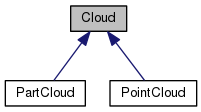
\includegraphics[width=223pt]{class_cloud__inherit__graph}
\end{center}
\end{figure}
\subsection*{Public Types}
\begin{DoxyCompactItemize}
\item 
typedef std\-::unique\-\_\-ptr$<$ \hyperlink{class_cloud}{Cloud} $>$ \hyperlink{class_cloud_a8460ff60db0a23f3679fc830db160e2a}{Ptr}
\begin{DoxyCompactList}\small\item\em Pointer. \end{DoxyCompactList}\end{DoxyCompactItemize}
\subsection*{Public Attributes}
\begin{DoxyCompactItemize}
\item 
hop3d\-::\-U64 \hyperlink{class_cloud_aa89d2de77505b1a09032fe8317d7703c}{I\-D}
\end{DoxyCompactItemize}


\subsection{Member Typedef Documentation}
\hypertarget{class_cloud_a8460ff60db0a23f3679fc830db160e2a}{\index{Cloud@{Cloud}!Ptr@{Ptr}}
\index{Ptr@{Ptr}!Cloud@{Cloud}}
\subsubsection[{Ptr}]{\setlength{\rightskip}{0pt plus 5cm}typedef std\-::unique\-\_\-ptr$<${\bf Cloud}$>$ {\bf Cloud\-::\-Ptr}}}\label{class_cloud_a8460ff60db0a23f3679fc830db160e2a}


Pointer. 



\subsection{Member Data Documentation}
\hypertarget{class_cloud_aa89d2de77505b1a09032fe8317d7703c}{\index{Cloud@{Cloud}!I\-D@{I\-D}}
\index{I\-D@{I\-D}!Cloud@{Cloud}}
\subsubsection[{I\-D}]{\setlength{\rightskip}{0pt plus 5cm}hop3d\-::\-U64 Cloud\-::\-I\-D}}\label{class_cloud_aa89d2de77505b1a09032fe8317d7703c}


The documentation for this class was generated from the following file\-:\begin{DoxyCompactItemize}
\item 
include/\-Data/\hyperlink{_cloud_8h}{Cloud.\-h}\end{DoxyCompactItemize}

\hypertarget{class_graph_builder}{\section{Graph\-Builder Class Reference}
\label{class_graph_builder}\index{Graph\-Builder@{Graph\-Builder}}
}


{\ttfamily \#include $<$Graph\-Builder.\-h$>$}

\subsection*{Public Types}
\begin{DoxyCompactItemize}
\item 
typedef std\-::unique\-\_\-ptr\\*
$<$ \hyperlink{class_graph_builder}{Graph\-Builder} $>$ \hyperlink{class_graph_builder_a2bce26be1d5bfac38d3f69f4bf79217b}{Ptr}
\begin{DoxyCompactList}\small\item\em Pointer. \end{DoxyCompactList}\end{DoxyCompactItemize}


\subsection{Member Typedef Documentation}
\hypertarget{class_graph_builder_a2bce26be1d5bfac38d3f69f4bf79217b}{\index{Graph\-Builder@{Graph\-Builder}!Ptr@{Ptr}}
\index{Ptr@{Ptr}!GraphBuilder@{Graph\-Builder}}
\subsubsection[{Ptr}]{\setlength{\rightskip}{0pt plus 5cm}typedef std\-::unique\-\_\-ptr$<${\bf Graph\-Builder}$>$ {\bf Graph\-Builder\-::\-Ptr}}}\label{class_graph_builder_a2bce26be1d5bfac38d3f69f4bf79217b}


Pointer. 



The documentation for this class was generated from the following file\-:\begin{DoxyCompactItemize}
\item 
include/\-Core/\hyperlink{_graph_builder_8h}{Graph\-Builder.\-h}\end{DoxyCompactItemize}

\hypertarget{class_layer_filterer}{\section{Layer\-Filterer Class Reference}
\label{class_layer_filterer}\index{Layer\-Filterer@{Layer\-Filterer}}
}


{\ttfamily \#include $<$Layer\-Filterer.\-h$>$}

\subsection*{Public Types}
\begin{DoxyCompactItemize}
\item 
typedef std\-::unique\-\_\-ptr\\*
$<$ \hyperlink{class_layer_filterer}{Layer\-Filterer} $>$ \hyperlink{class_layer_filterer_af5e176ab8326c56ad59ef2db5216967f}{Ptr}
\begin{DoxyCompactList}\small\item\em Pointer. \end{DoxyCompactList}\end{DoxyCompactItemize}


\subsection{Member Typedef Documentation}
\hypertarget{class_layer_filterer_af5e176ab8326c56ad59ef2db5216967f}{\index{Layer\-Filterer@{Layer\-Filterer}!Ptr@{Ptr}}
\index{Ptr@{Ptr}!LayerFilterer@{Layer\-Filterer}}
\subsubsection[{Ptr}]{\setlength{\rightskip}{0pt plus 5cm}typedef std\-::unique\-\_\-ptr$<${\bf Layer\-Filterer}$>$ {\bf Layer\-Filterer\-::\-Ptr}}}\label{class_layer_filterer_af5e176ab8326c56ad59ef2db5216967f}


Pointer. 



The documentation for this class was generated from the following file\-:\begin{DoxyCompactItemize}
\item 
include/\-Core/\hyperlink{_layer_filterer_8h}{Layer\-Filterer.\-h}\end{DoxyCompactItemize}

\hypertarget{class_layer_vocabulary}{\section{Layer\-Vocabulary Class Reference}
\label{class_layer_vocabulary}\index{Layer\-Vocabulary@{Layer\-Vocabulary}}
}


{\ttfamily \#include $<$Vocabulary.\-h$>$}



Inheritance diagram for Layer\-Vocabulary\-:\nopagebreak
\begin{figure}[H]
\begin{center}
\leavevmode
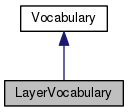
\includegraphics[width=168pt]{class_layer_vocabulary__inherit__graph}
\end{center}
\end{figure}


Collaboration diagram for Layer\-Vocabulary\-:\nopagebreak
\begin{figure}[H]
\begin{center}
\leavevmode
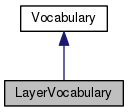
\includegraphics[width=168pt]{class_layer_vocabulary__coll__graph}
\end{center}
\end{figure}
\subsection*{Public Types}
\begin{DoxyCompactItemize}
\item 
typedef std\-::unique\-\_\-ptr\\*
$<$ \hyperlink{class_layer_vocabulary}{Layer\-Vocabulary} $>$ \hyperlink{class_layer_vocabulary_adc324deadcd03d2844a300b98421a39b}{Ptr}
\begin{DoxyCompactList}\small\item\em Pointer. \end{DoxyCompactList}\end{DoxyCompactItemize}


\subsection{Member Typedef Documentation}
\hypertarget{class_layer_vocabulary_adc324deadcd03d2844a300b98421a39b}{\index{Layer\-Vocabulary@{Layer\-Vocabulary}!Ptr@{Ptr}}
\index{Ptr@{Ptr}!LayerVocabulary@{Layer\-Vocabulary}}
\subsubsection[{Ptr}]{\setlength{\rightskip}{0pt plus 5cm}typedef std\-::unique\-\_\-ptr$<${\bf Layer\-Vocabulary}$>$ {\bf Layer\-Vocabulary\-::\-Ptr}}}\label{class_layer_vocabulary_adc324deadcd03d2844a300b98421a39b}


Pointer. 



The documentation for this class was generated from the following file\-:\begin{DoxyCompactItemize}
\item 
include/\-Data/\hyperlink{_vocabulary_8h}{Vocabulary.\-h}\end{DoxyCompactItemize}

\hypertarget{class_local_inhibiter}{\section{Local\-Inhibiter Class Reference}
\label{class_local_inhibiter}\index{Local\-Inhibiter@{Local\-Inhibiter}}
}


{\ttfamily \#include $<$Local\-Inhibiter.\-h$>$}

\subsection*{Public Types}
\begin{DoxyCompactItemize}
\item 
typedef std\-::unique\-\_\-ptr\\*
$<$ \hyperlink{class_local_inhibiter}{Local\-Inhibiter} $>$ \hyperlink{class_local_inhibiter_adb0900eb28d67eb178802c68d307e070}{Ptr}
\begin{DoxyCompactList}\small\item\em Pointer. \end{DoxyCompactList}\end{DoxyCompactItemize}


\subsection{Member Typedef Documentation}
\hypertarget{class_local_inhibiter_adb0900eb28d67eb178802c68d307e070}{\index{Local\-Inhibiter@{Local\-Inhibiter}!Ptr@{Ptr}}
\index{Ptr@{Ptr}!LocalInhibiter@{Local\-Inhibiter}}
\subsubsection[{Ptr}]{\setlength{\rightskip}{0pt plus 5cm}typedef std\-::unique\-\_\-ptr$<${\bf Local\-Inhibiter}$>$ {\bf Local\-Inhibiter\-::\-Ptr}}}\label{class_local_inhibiter_adb0900eb28d67eb178802c68d307e070}


Pointer. 



The documentation for this class was generated from the following file\-:\begin{DoxyCompactItemize}
\item 
include/\-Core/\hyperlink{_local_inhibiter_8h}{Local\-Inhibiter.\-h}\end{DoxyCompactItemize}

\hypertarget{class_object_graph}{\section{Object\-Graph Class Reference}
\label{class_object_graph}\index{Object\-Graph@{Object\-Graph}}
}


{\ttfamily \#include $<$Graph.\-h$>$}

\subsection*{Public Types}
\begin{DoxyCompactItemize}
\item 
typedef std\-::unique\-\_\-ptr\\*
$<$ \hyperlink{class_object_graph}{Object\-Graph} $>$ \hyperlink{class_object_graph_ad2359e9fe0859848c13b72155fba324f}{Ptr}
\begin{DoxyCompactList}\small\item\em Pointer. \end{DoxyCompactList}\end{DoxyCompactItemize}


\subsection{Member Typedef Documentation}
\hypertarget{class_object_graph_ad2359e9fe0859848c13b72155fba324f}{\index{Object\-Graph@{Object\-Graph}!Ptr@{Ptr}}
\index{Ptr@{Ptr}!ObjectGraph@{Object\-Graph}}
\subsubsection[{Ptr}]{\setlength{\rightskip}{0pt plus 5cm}typedef std\-::unique\-\_\-ptr$<${\bf Object\-Graph}$>$ {\bf Object\-Graph\-::\-Ptr}}}\label{class_object_graph_ad2359e9fe0859848c13b72155fba324f}


Pointer. 



The documentation for this class was generated from the following file\-:\begin{DoxyCompactItemize}
\item 
include/\-Data/\hyperlink{_graph_8h}{Graph.\-h}\end{DoxyCompactItemize}

\hypertarget{class_part}{\section{Part Class Reference}
\label{class_part}\index{Part@{Part}}
}


{\ttfamily \#include $<$Part.\-h$>$}



Inheritance diagram for Part\-:\nopagebreak
\begin{figure}[H]
\begin{center}
\leavevmode
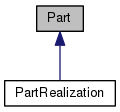
\includegraphics[width=162pt]{class_part__inherit__graph}
\end{center}
\end{figure}
\subsection*{Protected Types}
\begin{DoxyCompactItemize}
\item 
typedef std\-::unique\-\_\-ptr$<$ \hyperlink{class_part}{Part} $>$ \hyperlink{class_part_a270255868bbd294da6cdbe1a22fd71c0}{Ptr}
\begin{DoxyCompactList}\small\item\em Pointer. \end{DoxyCompactList}\item 
typedef std\-::vector$<$ \hyperlink{class_part}{Part} $>$ \hyperlink{class_part_a9cbb31df0bd4615cb133293acd55a938}{Seq}
\end{DoxyCompactItemize}
\subsection*{Protected Attributes}
\begin{DoxyCompactItemize}
\item 
hop3d\-::\-U64 \hyperlink{class_part_a3d19e990ee30d25cd5f12610864300db}{Id}
\item 
hop3d\-::\-U8 \hyperlink{class_part_ac4e9f24ead3926518a74b37c5101efc0}{Layer\-Id}
\item 
hop3d\-::\-U64 \hyperlink{class_part_a1dafacbc907066c3976ca09dc69a7421}{Central}
\item 
std\-::vector$<$ hop3d\-::\-U64 $>$ \hyperlink{class_part_ad5e3891ace1e60c4b0c9b86bad225a38}{Members}
\end{DoxyCompactItemize}
\subsection*{Friends}
\begin{DoxyCompactItemize}
\item 
class \hyperlink{class_part_a89d34d14776f6667e8cf4c088578f931}{Layer\-Vocabulary}
\end{DoxyCompactItemize}


\subsection{Member Typedef Documentation}
\hypertarget{class_part_a270255868bbd294da6cdbe1a22fd71c0}{\index{Part@{Part}!Ptr@{Ptr}}
\index{Ptr@{Ptr}!Part@{Part}}
\subsubsection[{Ptr}]{\setlength{\rightskip}{0pt plus 5cm}typedef std\-::unique\-\_\-ptr$<${\bf Part}$>$ {\bf Part\-::\-Ptr}\hspace{0.3cm}{\ttfamily [protected]}}}\label{class_part_a270255868bbd294da6cdbe1a22fd71c0}


Pointer. 

\hypertarget{class_part_a9cbb31df0bd4615cb133293acd55a938}{\index{Part@{Part}!Seq@{Seq}}
\index{Seq@{Seq}!Part@{Part}}
\subsubsection[{Seq}]{\setlength{\rightskip}{0pt plus 5cm}typedef std\-::vector$<${\bf Part}$>$ {\bf Part\-::\-Seq}\hspace{0.3cm}{\ttfamily [protected]}}}\label{class_part_a9cbb31df0bd4615cb133293acd55a938}


\subsection{Friends And Related Function Documentation}
\hypertarget{class_part_a89d34d14776f6667e8cf4c088578f931}{\index{Part@{Part}!Layer\-Vocabulary@{Layer\-Vocabulary}}
\index{Layer\-Vocabulary@{Layer\-Vocabulary}!Part@{Part}}
\subsubsection[{Layer\-Vocabulary}]{\setlength{\rightskip}{0pt plus 5cm}friend class {\bf Layer\-Vocabulary}\hspace{0.3cm}{\ttfamily [friend]}}}\label{class_part_a89d34d14776f6667e8cf4c088578f931}


\subsection{Member Data Documentation}
\hypertarget{class_part_a1dafacbc907066c3976ca09dc69a7421}{\index{Part@{Part}!Central@{Central}}
\index{Central@{Central}!Part@{Part}}
\subsubsection[{Central}]{\setlength{\rightskip}{0pt plus 5cm}hop3d\-::\-U64 Part\-::\-Central\hspace{0.3cm}{\ttfamily [protected]}}}\label{class_part_a1dafacbc907066c3976ca09dc69a7421}
\hypertarget{class_part_a3d19e990ee30d25cd5f12610864300db}{\index{Part@{Part}!Id@{Id}}
\index{Id@{Id}!Part@{Part}}
\subsubsection[{Id}]{\setlength{\rightskip}{0pt plus 5cm}hop3d\-::\-U64 Part\-::\-Id\hspace{0.3cm}{\ttfamily [protected]}}}\label{class_part_a3d19e990ee30d25cd5f12610864300db}
\hypertarget{class_part_ac4e9f24ead3926518a74b37c5101efc0}{\index{Part@{Part}!Layer\-Id@{Layer\-Id}}
\index{Layer\-Id@{Layer\-Id}!Part@{Part}}
\subsubsection[{Layer\-Id}]{\setlength{\rightskip}{0pt plus 5cm}hop3d\-::\-U8 Part\-::\-Layer\-Id\hspace{0.3cm}{\ttfamily [protected]}}}\label{class_part_ac4e9f24ead3926518a74b37c5101efc0}
\hypertarget{class_part_ad5e3891ace1e60c4b0c9b86bad225a38}{\index{Part@{Part}!Members@{Members}}
\index{Members@{Members}!Part@{Part}}
\subsubsection[{Members}]{\setlength{\rightskip}{0pt plus 5cm}std\-::vector$<$hop3d\-::\-U64$>$ Part\-::\-Members\hspace{0.3cm}{\ttfamily [protected]}}}\label{class_part_ad5e3891ace1e60c4b0c9b86bad225a38}


The documentation for this class was generated from the following file\-:\begin{DoxyCompactItemize}
\item 
include/\-Data/\hyperlink{_part_8h}{Part.\-h}\end{DoxyCompactItemize}

\hypertarget{class_part_cloud}{\section{Part\-Cloud Class Reference}
\label{class_part_cloud}\index{Part\-Cloud@{Part\-Cloud}}
}


{\ttfamily \#include $<$Cloud.\-h$>$}



Inheritance diagram for Part\-Cloud\-:\nopagebreak
\begin{figure}[H]
\begin{center}
\leavevmode
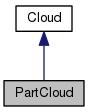
\includegraphics[width=138pt]{class_part_cloud__inherit__graph}
\end{center}
\end{figure}


Collaboration diagram for Part\-Cloud\-:\nopagebreak
\begin{figure}[H]
\begin{center}
\leavevmode
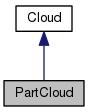
\includegraphics[width=138pt]{class_part_cloud__coll__graph}
\end{center}
\end{figure}
\subsection*{Public Types}
\begin{DoxyCompactItemize}
\item 
typedef std\-::unique\-\_\-ptr\\*
$<$ \hyperlink{class_part_cloud}{Part\-Cloud} $>$ \hyperlink{class_part_cloud_aec4e083f6d74ba725a554de89e56b170}{Ptr}
\begin{DoxyCompactList}\small\item\em Pointer. \end{DoxyCompactList}\end{DoxyCompactItemize}
\subsection*{Public Attributes}
\begin{DoxyCompactItemize}
\item 
std\-::vector$<$ \hyperlink{class_part_realization}{Part\-Realization} $>$ \hyperlink{class_part_cloud_a22d75c4d769cbf7223c429809de20641}{part\-Cloud}
\end{DoxyCompactItemize}


\subsection{Member Typedef Documentation}
\hypertarget{class_part_cloud_aec4e083f6d74ba725a554de89e56b170}{\index{Part\-Cloud@{Part\-Cloud}!Ptr@{Ptr}}
\index{Ptr@{Ptr}!PartCloud@{Part\-Cloud}}
\subsubsection[{Ptr}]{\setlength{\rightskip}{0pt plus 5cm}typedef std\-::unique\-\_\-ptr$<${\bf Part\-Cloud}$>$ {\bf Part\-Cloud\-::\-Ptr}}}\label{class_part_cloud_aec4e083f6d74ba725a554de89e56b170}


Pointer. 



\subsection{Member Data Documentation}
\hypertarget{class_part_cloud_a22d75c4d769cbf7223c429809de20641}{\index{Part\-Cloud@{Part\-Cloud}!part\-Cloud@{part\-Cloud}}
\index{part\-Cloud@{part\-Cloud}!PartCloud@{Part\-Cloud}}
\subsubsection[{part\-Cloud}]{\setlength{\rightskip}{0pt plus 5cm}std\-::vector$<${\bf Part\-Realization}$>$ Part\-Cloud\-::part\-Cloud}}\label{class_part_cloud_a22d75c4d769cbf7223c429809de20641}


The documentation for this class was generated from the following file\-:\begin{DoxyCompactItemize}
\item 
include/\-Data/\hyperlink{_cloud_8h}{Cloud.\-h}\end{DoxyCompactItemize}

\hypertarget{class_part_realization}{\section{Part\-Realization Class Reference}
\label{class_part_realization}\index{Part\-Realization@{Part\-Realization}}
}


{\ttfamily \#include $<$Part.\-h$>$}



Inheritance diagram for Part\-Realization\-:\nopagebreak
\begin{figure}[H]
\begin{center}
\leavevmode
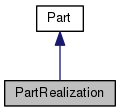
\includegraphics[width=162pt]{class_part_realization__inherit__graph}
\end{center}
\end{figure}


Collaboration diagram for Part\-Realization\-:\nopagebreak
\begin{figure}[H]
\begin{center}
\leavevmode
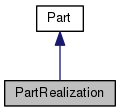
\includegraphics[width=162pt]{class_part_realization__coll__graph}
\end{center}
\end{figure}
\subsection*{Public Types}
\begin{DoxyCompactItemize}
\item 
typedef std\-::unique\-\_\-ptr\\*
$<$ \hyperlink{class_part_realization}{Part\-Realization} $>$ \hyperlink{class_part_realization_aec2d1af3a61dba0792d0d95bf32e7118}{Ptr}
\begin{DoxyCompactList}\small\item\em Pointer. \end{DoxyCompactList}\item 
typedef std\-::vector\\*
$<$ \hyperlink{class_part_realization}{Part\-Realization} $>$ \hyperlink{class_part_realization_ac53d0830ece33a44aaf825f109e00f59}{Seq}
\end{DoxyCompactItemize}
\subsection*{Public Attributes}
\begin{DoxyCompactItemize}
\item 
hop3d\-::\-Position \hyperlink{class_part_realization_a64e569cf60fcec7d6e31c47ea0a46e6e}{position}
\item 
hop3d\-::\-Reference\-Frame \hyperlink{class_part_realization_a31f7d192d8e527643997fa79aba5c28c}{reference\-Frame}
\item 
hop3d\-::\-F32 \hyperlink{class_part_realization_a814790d0300a7f1b3be036031e92fec0}{Activation}
\item 
hop3d\-::\-I8 \hyperlink{class_part_realization_acd7a731093a911fc165649d1a4baa96d}{Scale}
\end{DoxyCompactItemize}


\subsection{Member Typedef Documentation}
\hypertarget{class_part_realization_aec2d1af3a61dba0792d0d95bf32e7118}{\index{Part\-Realization@{Part\-Realization}!Ptr@{Ptr}}
\index{Ptr@{Ptr}!PartRealization@{Part\-Realization}}
\subsubsection[{Ptr}]{\setlength{\rightskip}{0pt plus 5cm}typedef std\-::unique\-\_\-ptr$<${\bf Part\-Realization}$>$ {\bf Part\-Realization\-::\-Ptr}}}\label{class_part_realization_aec2d1af3a61dba0792d0d95bf32e7118}


Pointer. 

\hypertarget{class_part_realization_ac53d0830ece33a44aaf825f109e00f59}{\index{Part\-Realization@{Part\-Realization}!Seq@{Seq}}
\index{Seq@{Seq}!PartRealization@{Part\-Realization}}
\subsubsection[{Seq}]{\setlength{\rightskip}{0pt plus 5cm}typedef std\-::vector$<${\bf Part\-Realization}$>$ {\bf Part\-Realization\-::\-Seq}}}\label{class_part_realization_ac53d0830ece33a44aaf825f109e00f59}


\subsection{Member Data Documentation}
\hypertarget{class_part_realization_a814790d0300a7f1b3be036031e92fec0}{\index{Part\-Realization@{Part\-Realization}!Activation@{Activation}}
\index{Activation@{Activation}!PartRealization@{Part\-Realization}}
\subsubsection[{Activation}]{\setlength{\rightskip}{0pt plus 5cm}hop3d\-::\-F32 Part\-Realization\-::\-Activation}}\label{class_part_realization_a814790d0300a7f1b3be036031e92fec0}
\hypertarget{class_part_realization_a64e569cf60fcec7d6e31c47ea0a46e6e}{\index{Part\-Realization@{Part\-Realization}!position@{position}}
\index{position@{position}!PartRealization@{Part\-Realization}}
\subsubsection[{position}]{\setlength{\rightskip}{0pt plus 5cm}hop3d\-::\-Position Part\-Realization\-::position}}\label{class_part_realization_a64e569cf60fcec7d6e31c47ea0a46e6e}
\hypertarget{class_part_realization_a31f7d192d8e527643997fa79aba5c28c}{\index{Part\-Realization@{Part\-Realization}!reference\-Frame@{reference\-Frame}}
\index{reference\-Frame@{reference\-Frame}!PartRealization@{Part\-Realization}}
\subsubsection[{reference\-Frame}]{\setlength{\rightskip}{0pt plus 5cm}hop3d\-::\-Reference\-Frame Part\-Realization\-::reference\-Frame}}\label{class_part_realization_a31f7d192d8e527643997fa79aba5c28c}
\hypertarget{class_part_realization_acd7a731093a911fc165649d1a4baa96d}{\index{Part\-Realization@{Part\-Realization}!Scale@{Scale}}
\index{Scale@{Scale}!PartRealization@{Part\-Realization}}
\subsubsection[{Scale}]{\setlength{\rightskip}{0pt plus 5cm}hop3d\-::\-I8 Part\-Realization\-::\-Scale}}\label{class_part_realization_acd7a731093a911fc165649d1a4baa96d}


The documentation for this class was generated from the following file\-:\begin{DoxyCompactItemize}
\item 
include/\-Data/\hyperlink{_part_8h}{Part.\-h}\end{DoxyCompactItemize}

\hypertarget{class_part_selector}{\section{Part\-Selector Class Reference}
\label{class_part_selector}\index{Part\-Selector@{Part\-Selector}}
}


{\ttfamily \#include $<$Part\-Selector.\-h$>$}

\subsection*{Public Types}
\begin{DoxyCompactItemize}
\item 
typedef std\-::unique\-\_\-ptr\\*
$<$ \hyperlink{class_part_selector}{Part\-Selector} $>$ \hyperlink{class_part_selector_a4fcdf24aa0af46b18de0bc5fde066e81}{Ptr}
\begin{DoxyCompactList}\small\item\em Pointer. \end{DoxyCompactList}\end{DoxyCompactItemize}


\subsection{Member Typedef Documentation}
\hypertarget{class_part_selector_a4fcdf24aa0af46b18de0bc5fde066e81}{\index{Part\-Selector@{Part\-Selector}!Ptr@{Ptr}}
\index{Ptr@{Ptr}!PartSelector@{Part\-Selector}}
\subsubsection[{Ptr}]{\setlength{\rightskip}{0pt plus 5cm}typedef std\-::unique\-\_\-ptr$<${\bf Part\-Selector}$>$ {\bf Part\-Selector\-::\-Ptr}}}\label{class_part_selector_a4fcdf24aa0af46b18de0bc5fde066e81}


Pointer. 



The documentation for this class was generated from the following file\-:\begin{DoxyCompactItemize}
\item 
include/\-Core/\hyperlink{_part_selector_8h}{Part\-Selector.\-h}\end{DoxyCompactItemize}

\hypertarget{class_point_cloud}{\section{Point\-Cloud Class Reference}
\label{class_point_cloud}\index{Point\-Cloud@{Point\-Cloud}}
}


{\ttfamily \#include $<$Cloud.\-h$>$}



Inheritance diagram for Point\-Cloud\-:\nopagebreak
\begin{figure}[H]
\begin{center}
\leavevmode
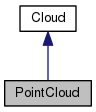
\includegraphics[width=144pt]{class_point_cloud__inherit__graph}
\end{center}
\end{figure}


Collaboration diagram for Point\-Cloud\-:\nopagebreak
\begin{figure}[H]
\begin{center}
\leavevmode
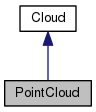
\includegraphics[width=144pt]{class_point_cloud__coll__graph}
\end{center}
\end{figure}
\subsection*{Public Types}
\begin{DoxyCompactItemize}
\item 
typedef std\-::unique\-\_\-ptr\\*
$<$ \hyperlink{class_point_cloud}{Point\-Cloud} $>$ \hyperlink{class_point_cloud_a150100920ea0a97f6867259251683256}{Ptr}
\begin{DoxyCompactList}\small\item\em Pointer. \end{DoxyCompactList}\end{DoxyCompactItemize}
\subsection*{Public Attributes}
\begin{DoxyCompactItemize}
\item 
std\-::vector$<$ hop3d\-::\-Point\-Normal $>$ \hyperlink{class_point_cloud_a96c71850c381b10db6a01ff979f1b6a5}{Point\-Cloud\-Normal}
\end{DoxyCompactItemize}


\subsection{Member Typedef Documentation}
\hypertarget{class_point_cloud_a150100920ea0a97f6867259251683256}{\index{Point\-Cloud@{Point\-Cloud}!Ptr@{Ptr}}
\index{Ptr@{Ptr}!PointCloud@{Point\-Cloud}}
\subsubsection[{Ptr}]{\setlength{\rightskip}{0pt plus 5cm}typedef std\-::unique\-\_\-ptr$<${\bf Point\-Cloud}$>$ {\bf Point\-Cloud\-::\-Ptr}}}\label{class_point_cloud_a150100920ea0a97f6867259251683256}


Pointer. 



\subsection{Member Data Documentation}
\hypertarget{class_point_cloud_a96c71850c381b10db6a01ff979f1b6a5}{\index{Point\-Cloud@{Point\-Cloud}!Point\-Cloud\-Normal@{Point\-Cloud\-Normal}}
\index{Point\-Cloud\-Normal@{Point\-Cloud\-Normal}!PointCloud@{Point\-Cloud}}
\subsubsection[{Point\-Cloud\-Normal}]{\setlength{\rightskip}{0pt plus 5cm}std\-::vector$<$hop3d\-::\-Point\-Normal$>$ Point\-Cloud\-::\-Point\-Cloud\-Normal}}\label{class_point_cloud_a96c71850c381b10db6a01ff979f1b6a5}


The documentation for this class was generated from the following file\-:\begin{DoxyCompactItemize}
\item 
include/\-Data/\hyperlink{_cloud_8h}{Cloud.\-h}\end{DoxyCompactItemize}

\hypertarget{class_reader}{\section{Reader Class Reference}
\label{class_reader}\index{Reader@{Reader}}
}


{\ttfamily \#include $<$Reader.\-h$>$}

\subsection*{Public Types}
\begin{DoxyCompactItemize}
\item 
typedef std\-::unique\-\_\-ptr$<$ \hyperlink{class_reader}{Reader} $>$ \hyperlink{class_reader_aca9a3e7e4e5d47385235587c6f86c592}{Ptr}
\begin{DoxyCompactList}\small\item\em Pointer. \end{DoxyCompactList}\end{DoxyCompactItemize}
\subsection*{Public Member Functions}
\begin{DoxyCompactItemize}
\item 
int \hyperlink{class_reader_af6c9fb04a6f48959aaf11aa68a9c2a52}{read\-Ply\-File} (std\-::string file\-Name, \hyperlink{class_point_cloud}{Point\-Cloud} \&point\-Cloud, std\-::vector$<$ Eigen\-::\-Vector4i $>$ \&output\-Faces)
\end{DoxyCompactItemize}
\subsection*{Protected Member Functions}
\begin{DoxyCompactItemize}
\item 
void \hyperlink{class_reader_a6f5ad886644e606d7dda4e3ae6a37cdf}{split} (const std\-::string \&s, char c, std\-::vector$<$ std\-::string $>$ \&v)
\end{DoxyCompactItemize}


\subsection{Member Typedef Documentation}
\hypertarget{class_reader_aca9a3e7e4e5d47385235587c6f86c592}{\index{Reader@{Reader}!Ptr@{Ptr}}
\index{Ptr@{Ptr}!Reader@{Reader}}
\subsubsection[{Ptr}]{\setlength{\rightskip}{0pt plus 5cm}typedef std\-::unique\-\_\-ptr$<${\bf Reader}$>$ {\bf Reader\-::\-Ptr}}}\label{class_reader_aca9a3e7e4e5d47385235587c6f86c592}


Pointer. 



\subsection{Member Function Documentation}
\hypertarget{class_reader_af6c9fb04a6f48959aaf11aa68a9c2a52}{\index{Reader@{Reader}!read\-Ply\-File@{read\-Ply\-File}}
\index{read\-Ply\-File@{read\-Ply\-File}!Reader@{Reader}}
\subsubsection[{read\-Ply\-File}]{\setlength{\rightskip}{0pt plus 5cm}int Reader\-::read\-Ply\-File (
\begin{DoxyParamCaption}
\item[{std\-::string}]{file\-Name, }
\item[{{\bf Point\-Cloud} \&}]{point\-Cloud, }
\item[{std\-::vector$<$ Eigen\-::\-Vector4i $>$ \&}]{output\-Faces}
\end{DoxyParamCaption}
)}}\label{class_reader_af6c9fb04a6f48959aaf11aa68a9c2a52}
\hypertarget{class_reader_a6f5ad886644e606d7dda4e3ae6a37cdf}{\index{Reader@{Reader}!split@{split}}
\index{split@{split}!Reader@{Reader}}
\subsubsection[{split}]{\setlength{\rightskip}{0pt plus 5cm}void Reader\-::split (
\begin{DoxyParamCaption}
\item[{const std\-::string \&}]{s, }
\item[{char}]{c, }
\item[{std\-::vector$<$ std\-::string $>$ \&}]{v}
\end{DoxyParamCaption}
)\hspace{0.3cm}{\ttfamily [protected]}}}\label{class_reader_a6f5ad886644e606d7dda4e3ae6a37cdf}


The documentation for this class was generated from the following files\-:\begin{DoxyCompactItemize}
\item 
include/\-Utilities/\hyperlink{_reader_8h}{Reader.\-h}\item 
src/\-Utilities/\hyperlink{_reader_8cpp}{Reader.\-cpp}\end{DoxyCompactItemize}

\hypertarget{class_statistics_builder}{\section{Statistics\-Builder Class Reference}
\label{class_statistics_builder}\index{Statistics\-Builder@{Statistics\-Builder}}
}


{\ttfamily \#include $<$Statistics\-Builder.\-h$>$}

\subsection*{Public Types}
\begin{DoxyCompactItemize}
\item 
typedef std\-::unique\-\_\-ptr\\*
$<$ \hyperlink{class_statistics_builder}{Statistics\-Builder} $>$ \hyperlink{class_statistics_builder_a004e4a71362f6accecdb3504ee328aa6}{Ptr}
\begin{DoxyCompactList}\small\item\em Pointer. \end{DoxyCompactList}\end{DoxyCompactItemize}


\subsection{Member Typedef Documentation}
\hypertarget{class_statistics_builder_a004e4a71362f6accecdb3504ee328aa6}{\index{Statistics\-Builder@{Statistics\-Builder}!Ptr@{Ptr}}
\index{Ptr@{Ptr}!StatisticsBuilder@{Statistics\-Builder}}
\subsubsection[{Ptr}]{\setlength{\rightskip}{0pt plus 5cm}typedef std\-::unique\-\_\-ptr$<${\bf Statistics\-Builder}$>$ {\bf Statistics\-Builder\-::\-Ptr}}}\label{class_statistics_builder_a004e4a71362f6accecdb3504ee328aa6}


Pointer. 



The documentation for this class was generated from the following file\-:\begin{DoxyCompactItemize}
\item 
include/\-Core/\hyperlink{_statistics_builder_8h}{Statistics\-Builder.\-h}\end{DoxyCompactItemize}

\hypertarget{class_vocabulary}{\section{Vocabulary Class Reference}
\label{class_vocabulary}\index{Vocabulary@{Vocabulary}}
}


{\ttfamily \#include $<$Vocabulary.\-h$>$}

\subsection*{Public Types}
\begin{DoxyCompactItemize}
\item 
typedef std\-::unique\-\_\-ptr\\*
$<$ \hyperlink{class_vocabulary}{Vocabulary} $>$ \hyperlink{class_vocabulary_aaeaf17c4e25e6d7c8cb3ce9598c74715}{Ptr}
\begin{DoxyCompactList}\small\item\em Pointer. \end{DoxyCompactList}\end{DoxyCompactItemize}
\subsection*{Public Attributes}
\begin{DoxyCompactItemize}
\item 
\hyperlink{class_layer_vocabulary_a6098bd61090934286a749873181b5077}{Layer\-Vocabulary\-::\-Seq} \hyperlink{class_vocabulary_a773229c5a76412765f5e486c287bea88}{Learnt\-Vocabulary}
\end{DoxyCompactItemize}


\subsection{Member Typedef Documentation}
\hypertarget{class_vocabulary_aaeaf17c4e25e6d7c8cb3ce9598c74715}{\index{Vocabulary@{Vocabulary}!Ptr@{Ptr}}
\index{Ptr@{Ptr}!Vocabulary@{Vocabulary}}
\subsubsection[{Ptr}]{\setlength{\rightskip}{0pt plus 5cm}typedef std\-::unique\-\_\-ptr$<${\bf Vocabulary}$>$ {\bf Vocabulary\-::\-Ptr}}}\label{class_vocabulary_aaeaf17c4e25e6d7c8cb3ce9598c74715}


Pointer. 



\subsection{Member Data Documentation}
\hypertarget{class_vocabulary_a773229c5a76412765f5e486c287bea88}{\index{Vocabulary@{Vocabulary}!Learnt\-Vocabulary@{Learnt\-Vocabulary}}
\index{Learnt\-Vocabulary@{Learnt\-Vocabulary}!Vocabulary@{Vocabulary}}
\subsubsection[{Learnt\-Vocabulary}]{\setlength{\rightskip}{0pt plus 5cm}{\bf Layer\-Vocabulary\-::\-Seq} Vocabulary\-::\-Learnt\-Vocabulary}}\label{class_vocabulary_a773229c5a76412765f5e486c287bea88}


The documentation for this class was generated from the following file\-:\begin{DoxyCompactItemize}
\item 
include/\-Data/\hyperlink{_vocabulary_8h}{Vocabulary.\-h}\end{DoxyCompactItemize}

\hypertarget{class_writer}{\section{Writer Class Reference}
\label{class_writer}\index{Writer@{Writer}}
}


{\ttfamily \#include $<$Writer.\-h$>$}

\subsection*{Public Types}
\begin{DoxyCompactItemize}
\item 
typedef std\-::unique\-\_\-ptr$<$ \hyperlink{class_writer}{Writer} $>$ \hyperlink{class_writer_a969188b5d6bad75395bdd8a7fe4a6907}{Ptr}
\begin{DoxyCompactList}\small\item\em Pointer. \end{DoxyCompactList}\end{DoxyCompactItemize}


\subsection{Member Typedef Documentation}
\hypertarget{class_writer_a969188b5d6bad75395bdd8a7fe4a6907}{\index{Writer@{Writer}!Ptr@{Ptr}}
\index{Ptr@{Ptr}!Writer@{Writer}}
\subsubsection[{Ptr}]{\setlength{\rightskip}{0pt plus 5cm}typedef std\-::unique\-\_\-ptr$<${\bf Writer}$>$ {\bf Writer\-::\-Ptr}}}\label{class_writer_a969188b5d6bad75395bdd8a7fe4a6907}


Pointer. 



The documentation for this class was generated from the following file\-:\begin{DoxyCompactItemize}
\item 
include/\-Utilities/\hyperlink{_writer_8h}{Writer.\-h}\end{DoxyCompactItemize}

\chapter{File Documentation}
\hypertarget{_inference_2_data_8h}{\section{include/\-Apps/\-Inference/\-Data.h File Reference}
\label{_inference_2_data_8h}\index{include/\-Apps/\-Inference/\-Data.\-h@{include/\-Apps/\-Inference/\-Data.\-h}}
}

\hypertarget{_learning_2_data_8h}{\section{include/\-Apps/\-Learning/\-Data.h File Reference}
\label{_learning_2_data_8h}\index{include/\-Apps/\-Learning/\-Data.\-h@{include/\-Apps/\-Learning/\-Data.\-h}}
}

\hypertarget{_inference_8h}{\section{include/\-Apps/\-Inference/\-Inference.h File Reference}
\label{_inference_8h}\index{include/\-Apps/\-Inference/\-Inference.\-h@{include/\-Apps/\-Inference/\-Inference.\-h}}
}

\hypertarget{_learning_8h}{\section{include/\-Apps/\-Learning/\-Learning.h File Reference}
\label{_learning_8h}\index{include/\-Apps/\-Learning/\-Learning.\-h@{include/\-Apps/\-Learning/\-Learning.\-h}}
}

\hypertarget{_graph_builder_8h}{\section{include/\-Core/\-Graph\-Builder.h File Reference}
\label{_graph_builder_8h}\index{include/\-Core/\-Graph\-Builder.\-h@{include/\-Core/\-Graph\-Builder.\-h}}
}
{\ttfamily \#include $<$iostream$>$}\\*
{\ttfamily \#include $<$memory$>$}\\*
Include dependency graph for Graph\-Builder.\-h\-:\nopagebreak
\begin{figure}[H]
\begin{center}
\leavevmode
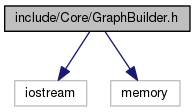
\includegraphics[width=218pt]{_graph_builder_8h__incl}
\end{center}
\end{figure}
This graph shows which files directly or indirectly include this file\-:\nopagebreak
\begin{figure}[H]
\begin{center}
\leavevmode
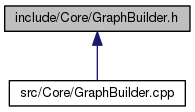
\includegraphics[width=218pt]{_graph_builder_8h__dep__incl}
\end{center}
\end{figure}
\subsection*{Classes}
\begin{DoxyCompactItemize}
\item 
class \hyperlink{class_graph_builder}{Graph\-Builder}
\end{DoxyCompactItemize}

\hypertarget{_layer_filterer_8h}{\section{include/\-Core/\-Layer\-Filterer.h File Reference}
\label{_layer_filterer_8h}\index{include/\-Core/\-Layer\-Filterer.\-h@{include/\-Core/\-Layer\-Filterer.\-h}}
}
{\ttfamily \#include $<$iostream$>$}\\*
{\ttfamily \#include $<$memory$>$}\\*
Include dependency graph for Layer\-Filterer.\-h\-:\nopagebreak
\begin{figure}[H]
\begin{center}
\leavevmode
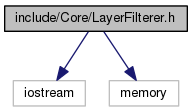
\includegraphics[width=216pt]{_layer_filterer_8h__incl}
\end{center}
\end{figure}
This graph shows which files directly or indirectly include this file\-:\nopagebreak
\begin{figure}[H]
\begin{center}
\leavevmode
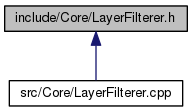
\includegraphics[width=216pt]{_layer_filterer_8h__dep__incl}
\end{center}
\end{figure}
\subsection*{Classes}
\begin{DoxyCompactItemize}
\item 
class \hyperlink{class_layer_filterer}{Layer\-Filterer}
\end{DoxyCompactItemize}

\hypertarget{_local_inhibiter_8h}{\section{include/\-Core/\-Local\-Inhibiter.h File Reference}
\label{_local_inhibiter_8h}\index{include/\-Core/\-Local\-Inhibiter.\-h@{include/\-Core/\-Local\-Inhibiter.\-h}}
}
{\ttfamily \#include $<$iostream$>$}\\*
{\ttfamily \#include $<$memory$>$}\\*
Include dependency graph for Local\-Inhibiter.\-h\-:\nopagebreak
\begin{figure}[H]
\begin{center}
\leavevmode
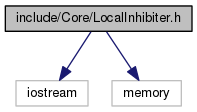
\includegraphics[width=220pt]{_local_inhibiter_8h__incl}
\end{center}
\end{figure}
This graph shows which files directly or indirectly include this file\-:\nopagebreak
\begin{figure}[H]
\begin{center}
\leavevmode
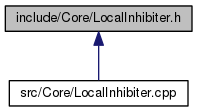
\includegraphics[width=220pt]{_local_inhibiter_8h__dep__incl}
\end{center}
\end{figure}
\subsection*{Classes}
\begin{DoxyCompactItemize}
\item 
class \hyperlink{class_local_inhibiter}{Local\-Inhibiter}
\end{DoxyCompactItemize}

\hypertarget{_part_selector_8h}{\section{include/\-Core/\-Part\-Selector.h File Reference}
\label{_part_selector_8h}\index{include/\-Core/\-Part\-Selector.\-h@{include/\-Core/\-Part\-Selector.\-h}}
}
{\ttfamily \#include $<$iostream$>$}\\*
{\ttfamily \#include $<$memory$>$}\\*
Include dependency graph for Part\-Selector.\-h\-:\nopagebreak
\begin{figure}[H]
\begin{center}
\leavevmode
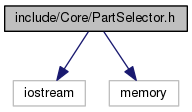
\includegraphics[width=216pt]{_part_selector_8h__incl}
\end{center}
\end{figure}
This graph shows which files directly or indirectly include this file\-:\nopagebreak
\begin{figure}[H]
\begin{center}
\leavevmode
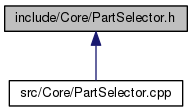
\includegraphics[width=216pt]{_part_selector_8h__dep__incl}
\end{center}
\end{figure}
\subsection*{Classes}
\begin{DoxyCompactItemize}
\item 
class \hyperlink{class_part_selector}{Part\-Selector}
\end{DoxyCompactItemize}

\hypertarget{_statistics_builder_8h}{\section{include/\-Core/\-Statistics\-Builder.h File Reference}
\label{_statistics_builder_8h}\index{include/\-Core/\-Statistics\-Builder.\-h@{include/\-Core/\-Statistics\-Builder.\-h}}
}
{\ttfamily \#include $<$iostream$>$}\\*
{\ttfamily \#include $<$memory$>$}\\*
Include dependency graph for Statistics\-Builder.\-h\-:\nopagebreak
\begin{figure}[H]
\begin{center}
\leavevmode
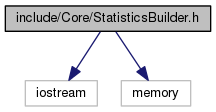
\includegraphics[width=234pt]{_statistics_builder_8h__incl}
\end{center}
\end{figure}
This graph shows which files directly or indirectly include this file\-:\nopagebreak
\begin{figure}[H]
\begin{center}
\leavevmode
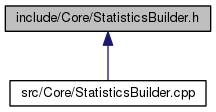
\includegraphics[width=234pt]{_statistics_builder_8h__dep__incl}
\end{center}
\end{figure}
\subsection*{Classes}
\begin{DoxyCompactItemize}
\item 
class \hyperlink{class_statistics_builder}{Statistics\-Builder}
\end{DoxyCompactItemize}

\hypertarget{_cloud_8h}{\section{include/\-Data/\-Cloud.h File Reference}
\label{_cloud_8h}\index{include/\-Data/\-Cloud.\-h@{include/\-Data/\-Cloud.\-h}}
}
{\ttfamily \#include $<$iostream$>$}\\*
{\ttfamily \#include $<$memory$>$}\\*
{\ttfamily \#include \char`\"{}Data/\-Defs.\-h\char`\"{}}\\*
{\ttfamily \#include \char`\"{}Data/\-Part.\-h\char`\"{}}\\*
Include dependency graph for Cloud.\-h\-:\nopagebreak
\begin{figure}[H]
\begin{center}
\leavevmode
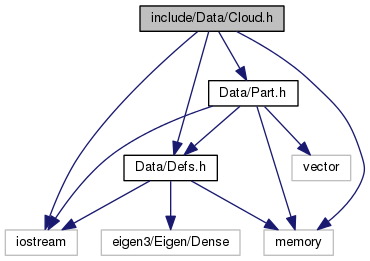
\includegraphics[width=349pt]{_cloud_8h__incl}
\end{center}
\end{figure}
This graph shows which files directly or indirectly include this file\-:\nopagebreak
\begin{figure}[H]
\begin{center}
\leavevmode
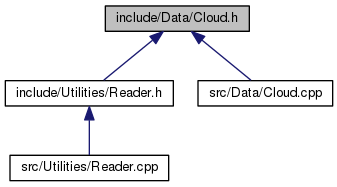
\includegraphics[width=325pt]{_cloud_8h__dep__incl}
\end{center}
\end{figure}
\subsection*{Classes}
\begin{DoxyCompactItemize}
\item 
class \hyperlink{class_cloud}{Cloud}
\item 
class \hyperlink{class_part_cloud}{Part\-Cloud}
\item 
class \hyperlink{class_point_cloud}{Point\-Cloud}
\end{DoxyCompactItemize}

\hypertarget{_defs_8h}{\section{include/\-Data/\-Defs.h File Reference}
\label{_defs_8h}\index{include/\-Data/\-Defs.\-h@{include/\-Data/\-Defs.\-h}}
}
{\ttfamily \#include $<$iostream$>$}\\*
{\ttfamily \#include $<$memory$>$}\\*
{\ttfamily \#include $<$eigen3/\-Eigen/\-Dense$>$}\\*
Include dependency graph for Defs.\-h\-:\nopagebreak
\begin{figure}[H]
\begin{center}
\leavevmode
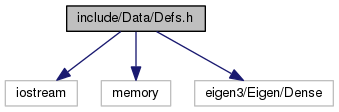
\includegraphics[width=326pt]{_defs_8h__incl}
\end{center}
\end{figure}
This graph shows which files directly or indirectly include this file\-:
\nopagebreak
\begin{figure}[H]
\begin{center}
\leavevmode
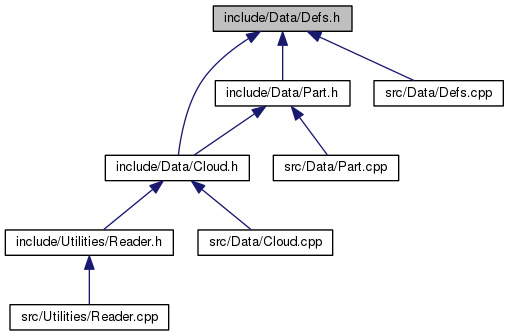
\includegraphics[width=350pt]{_defs_8h__dep__incl}
\end{center}
\end{figure}
\subsection*{Namespaces}
\begin{DoxyCompactItemize}
\item 
\hyperlink{namespacehop3d}{hop3d}
\end{DoxyCompactItemize}

\hypertarget{_graph_8h}{\section{include/\-Data/\-Graph.h File Reference}
\label{_graph_8h}\index{include/\-Data/\-Graph.\-h@{include/\-Data/\-Graph.\-h}}
}
{\ttfamily \#include $<$iostream$>$}\\*
{\ttfamily \#include $<$memory$>$}\\*
Include dependency graph for Graph.\-h\-:\nopagebreak
\begin{figure}[H]
\begin{center}
\leavevmode
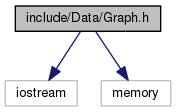
\includegraphics[width=204pt]{_graph_8h__incl}
\end{center}
\end{figure}
This graph shows which files directly or indirectly include this file\-:\nopagebreak
\begin{figure}[H]
\begin{center}
\leavevmode
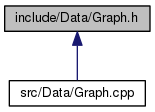
\includegraphics[width=188pt]{_graph_8h__dep__incl}
\end{center}
\end{figure}
\subsection*{Classes}
\begin{DoxyCompactItemize}
\item 
class \hyperlink{class_object_graph}{Object\-Graph}
\end{DoxyCompactItemize}

\hypertarget{_part_8h}{\section{include/\-Data/\-Part.h File Reference}
\label{_part_8h}\index{include/\-Data/\-Part.\-h@{include/\-Data/\-Part.\-h}}
}
{\ttfamily \#include $<$iostream$>$}\\*
{\ttfamily \#include $<$memory$>$}\\*
{\ttfamily \#include $<$vector$>$}\\*
{\ttfamily \#include \char`\"{}Data/\-Defs.\-h\char`\"{}}\\*
Include dependency graph for Part.\-h\-:\nopagebreak
\begin{figure}[H]
\begin{center}
\leavevmode
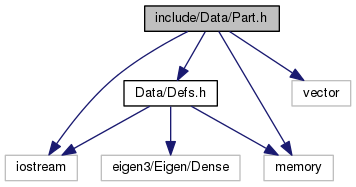
\includegraphics[width=339pt]{_part_8h__incl}
\end{center}
\end{figure}
This graph shows which files directly or indirectly include this file\-:\nopagebreak
\begin{figure}[H]
\begin{center}
\leavevmode
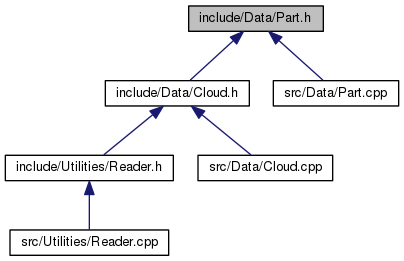
\includegraphics[width=350pt]{_part_8h__dep__incl}
\end{center}
\end{figure}
\subsection*{Classes}
\begin{DoxyCompactItemize}
\item 
class \hyperlink{class_part}{Part}
\item 
class \hyperlink{class_part_realization}{Part\-Realization}
\end{DoxyCompactItemize}

\hypertarget{_vocabulary_8h}{\section{include/\-Data/\-Vocabulary.h File Reference}
\label{_vocabulary_8h}\index{include/\-Data/\-Vocabulary.\-h@{include/\-Data/\-Vocabulary.\-h}}
}
{\ttfamily \#include $<$iostream$>$}\\*
{\ttfamily \#include $<$memory$>$}\\*
Include dependency graph for Vocabulary.\-h\-:\nopagebreak
\begin{figure}[H]
\begin{center}
\leavevmode
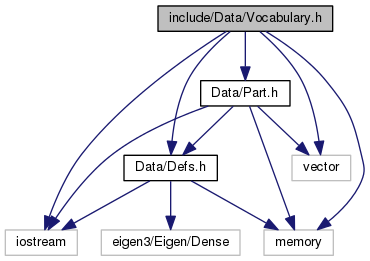
\includegraphics[width=210pt]{_vocabulary_8h__incl}
\end{center}
\end{figure}
This graph shows which files directly or indirectly include this file\-:\nopagebreak
\begin{figure}[H]
\begin{center}
\leavevmode
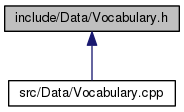
\includegraphics[width=210pt]{_vocabulary_8h__dep__incl}
\end{center}
\end{figure}
\subsection*{Classes}
\begin{DoxyCompactItemize}
\item 
class \hyperlink{class_vocabulary}{Vocabulary}
\item 
class \hyperlink{class_layer_vocabulary}{Layer\-Vocabulary}
\end{DoxyCompactItemize}

\hypertarget{_reader_8h}{\section{include/\-Utilities/\-Reader.h File Reference}
\label{_reader_8h}\index{include/\-Utilities/\-Reader.\-h@{include/\-Utilities/\-Reader.\-h}}
}
{\ttfamily \#include \char`\"{}Data/\-Cloud.\-h\char`\"{}}\\*
{\ttfamily \#include $<$iostream$>$}\\*
{\ttfamily \#include $<$memory$>$}\\*
{\ttfamily \#include $<$fstream$>$}\\*
{\ttfamily \#include $<$string$>$}\\*
Include dependency graph for Reader.\-h\-:\nopagebreak
\begin{figure}[H]
\begin{center}
\leavevmode
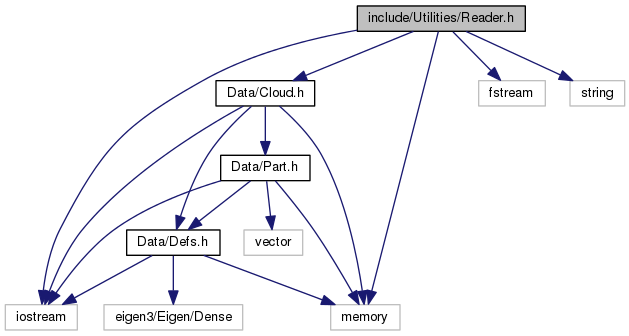
\includegraphics[width=350pt]{_reader_8h__incl}
\end{center}
\end{figure}
This graph shows which files directly or indirectly include this file\-:\nopagebreak
\begin{figure}[H]
\begin{center}
\leavevmode
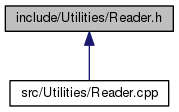
\includegraphics[width=206pt]{_reader_8h__dep__incl}
\end{center}
\end{figure}
\subsection*{Classes}
\begin{DoxyCompactItemize}
\item 
class \hyperlink{class_reader}{Reader}
\end{DoxyCompactItemize}

\hypertarget{_writer_8h}{\section{include/\-Utilities/\-Writer.h File Reference}
\label{_writer_8h}\index{include/\-Utilities/\-Writer.\-h@{include/\-Utilities/\-Writer.\-h}}
}
{\ttfamily \#include $<$iostream$>$}\\*
{\ttfamily \#include $<$memory$>$}\\*
Include dependency graph for Writer.\-h\-:\nopagebreak
\begin{figure}[H]
\begin{center}
\leavevmode
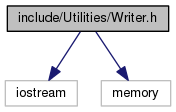
\includegraphics[width=204pt]{_writer_8h__incl}
\end{center}
\end{figure}
This graph shows which files directly or indirectly include this file\-:\nopagebreak
\begin{figure}[H]
\begin{center}
\leavevmode
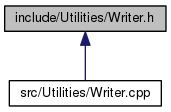
\includegraphics[width=200pt]{_writer_8h__dep__incl}
\end{center}
\end{figure}
\subsection*{Classes}
\begin{DoxyCompactItemize}
\item 
class \hyperlink{class_writer}{Writer}
\end{DoxyCompactItemize}

\hypertarget{main_8cpp}{\section{main.\-cpp File Reference}
\label{main_8cpp}\index{main.\-cpp@{main.\-cpp}}
}
{\ttfamily \#include $<$iostream$>$}\\*
Include dependency graph for main.\-cpp\-:\nopagebreak
\begin{figure}[H]
\begin{center}
\leavevmode
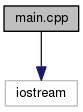
\includegraphics[width=134pt]{main_8cpp__incl}
\end{center}
\end{figure}
\subsection*{Functions}
\begin{DoxyCompactItemize}
\item 
int \hyperlink{main_8cpp_a3c04138a5bfe5d72780bb7e82a18e627}{main} (int argc, char $\ast$$\ast$argv)
\end{DoxyCompactItemize}


\subsection{Function Documentation}
\hypertarget{main_8cpp_a3c04138a5bfe5d72780bb7e82a18e627}{\index{main.\-cpp@{main.\-cpp}!main@{main}}
\index{main@{main}!main.cpp@{main.\-cpp}}
\subsubsection[{main}]{\setlength{\rightskip}{0pt plus 5cm}int main (
\begin{DoxyParamCaption}
\item[{int}]{argc, }
\item[{char $\ast$$\ast$}]{argv}
\end{DoxyParamCaption}
)}}\label{main_8cpp_a3c04138a5bfe5d72780bb7e82a18e627}

\hypertarget{_inference_2_data_8cpp}{\section{src/\-Apps/\-Inference/\-Data.cpp File Reference}
\label{_inference_2_data_8cpp}\index{src/\-Apps/\-Inference/\-Data.\-cpp@{src/\-Apps/\-Inference/\-Data.\-cpp}}
}

\hypertarget{_learning_2_data_8cpp}{\section{src/\-Apps/\-Learning/\-Data.cpp File Reference}
\label{_learning_2_data_8cpp}\index{src/\-Apps/\-Learning/\-Data.\-cpp@{src/\-Apps/\-Learning/\-Data.\-cpp}}
}

\hypertarget{_inference_8cpp}{\section{src/\-Apps/\-Inference/\-Inference.cpp File Reference}
\label{_inference_8cpp}\index{src/\-Apps/\-Inference/\-Inference.\-cpp@{src/\-Apps/\-Inference/\-Inference.\-cpp}}
}

\hypertarget{_learning_8cpp}{\section{src/\-Apps/\-Learning/\-Learning.cpp File Reference}
\label{_learning_8cpp}\index{src/\-Apps/\-Learning/\-Learning.\-cpp@{src/\-Apps/\-Learning/\-Learning.\-cpp}}
}

\hypertarget{_graph_builder_8cpp}{\section{src/\-Core/\-Graph\-Builder.cpp File Reference}
\label{_graph_builder_8cpp}\index{src/\-Core/\-Graph\-Builder.\-cpp@{src/\-Core/\-Graph\-Builder.\-cpp}}
}
{\ttfamily \#include \char`\"{}Core/\-Graph\-Builder.\-h\char`\"{}}\\*
Include dependency graph for Graph\-Builder.\-cpp\-:\nopagebreak
\begin{figure}[H]
\begin{center}
\leavevmode
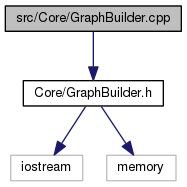
\includegraphics[width=212pt]{_graph_builder_8cpp__incl}
\end{center}
\end{figure}

\hypertarget{_layer_filterer_8cpp}{\section{src/\-Core/\-Layer\-Filterer.cpp File Reference}
\label{_layer_filterer_8cpp}\index{src/\-Core/\-Layer\-Filterer.\-cpp@{src/\-Core/\-Layer\-Filterer.\-cpp}}
}
{\ttfamily \#include \char`\"{}Core/\-Layer\-Filterer.\-h\char`\"{}}\\*
Include dependency graph for Layer\-Filterer.\-cpp\-:\nopagebreak
\begin{figure}[H]
\begin{center}
\leavevmode
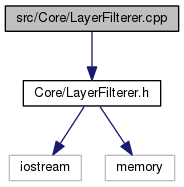
\includegraphics[width=210pt]{_layer_filterer_8cpp__incl}
\end{center}
\end{figure}

\hypertarget{_local_inhibiter_8cpp}{\section{src/\-Core/\-Local\-Inhibiter.cpp File Reference}
\label{_local_inhibiter_8cpp}\index{src/\-Core/\-Local\-Inhibiter.\-cpp@{src/\-Core/\-Local\-Inhibiter.\-cpp}}
}
{\ttfamily \#include \char`\"{}Core/\-Local\-Inhibiter.\-h\char`\"{}}\\*
Include dependency graph for Local\-Inhibiter.\-cpp\-:\nopagebreak
\begin{figure}[H]
\begin{center}
\leavevmode
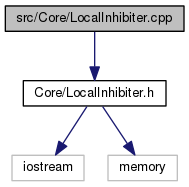
\includegraphics[width=214pt]{_local_inhibiter_8cpp__incl}
\end{center}
\end{figure}

\hypertarget{_part_selector_8cpp}{\section{src/\-Core/\-Part\-Selector.cpp File Reference}
\label{_part_selector_8cpp}\index{src/\-Core/\-Part\-Selector.\-cpp@{src/\-Core/\-Part\-Selector.\-cpp}}
}
{\ttfamily \#include \char`\"{}Core/\-Part\-Selector.\-h\char`\"{}}\\*
Include dependency graph for Part\-Selector.\-cpp\-:\nopagebreak
\begin{figure}[H]
\begin{center}
\leavevmode
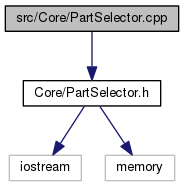
\includegraphics[width=210pt]{_part_selector_8cpp__incl}
\end{center}
\end{figure}

\hypertarget{_statistics_builder_8cpp}{\section{src/\-Core/\-Statistics\-Builder.cpp File Reference}
\label{_statistics_builder_8cpp}\index{src/\-Core/\-Statistics\-Builder.\-cpp@{src/\-Core/\-Statistics\-Builder.\-cpp}}
}
{\ttfamily \#include \char`\"{}Core/\-Statistics\-Builder.\-h\char`\"{}}\\*
Include dependency graph for Statistics\-Builder.\-cpp\-:\nopagebreak
\begin{figure}[H]
\begin{center}
\leavevmode
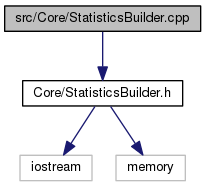
\includegraphics[width=226pt]{_statistics_builder_8cpp__incl}
\end{center}
\end{figure}

\hypertarget{_cloud_8cpp}{\section{src/\-Data/\-Cloud.cpp File Reference}
\label{_cloud_8cpp}\index{src/\-Data/\-Cloud.\-cpp@{src/\-Data/\-Cloud.\-cpp}}
}
{\ttfamily \#include \char`\"{}Data/\-Cloud.\-h\char`\"{}}\\*
Include dependency graph for Cloud.\-cpp\-:\nopagebreak
\begin{figure}[H]
\begin{center}
\leavevmode
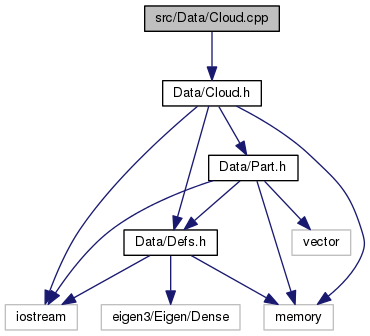
\includegraphics[width=349pt]{_cloud_8cpp__incl}
\end{center}
\end{figure}

\hypertarget{_defs_8cpp}{\section{src/\-Data/\-Defs.cpp File Reference}
\label{_defs_8cpp}\index{src/\-Data/\-Defs.\-cpp@{src/\-Data/\-Defs.\-cpp}}
}
{\ttfamily \#include \char`\"{}Data/\-Defs.\-h\char`\"{}}\\*
Include dependency graph for Defs.\-cpp\-:\nopagebreak
\begin{figure}[H]
\begin{center}
\leavevmode
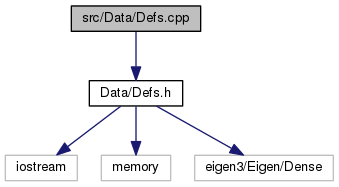
\includegraphics[width=326pt]{_defs_8cpp__incl}
\end{center}
\end{figure}

\hypertarget{_graph_8cpp}{\section{src/\-Data/\-Graph.cpp File Reference}
\label{_graph_8cpp}\index{src/\-Data/\-Graph.\-cpp@{src/\-Data/\-Graph.\-cpp}}
}
{\ttfamily \#include \char`\"{}Data/\-Graph.\-h\char`\"{}}\\*
Include dependency graph for Graph.\-cpp\-:\nopagebreak
\begin{figure}[H]
\begin{center}
\leavevmode
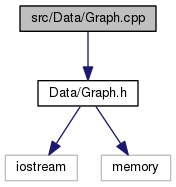
\includegraphics[width=204pt]{_graph_8cpp__incl}
\end{center}
\end{figure}

\hypertarget{_part_8cpp}{\section{src/\-Data/\-Part.cpp File Reference}
\label{_part_8cpp}\index{src/\-Data/\-Part.\-cpp@{src/\-Data/\-Part.\-cpp}}
}
{\ttfamily \#include \char`\"{}Data/\-Part.\-h\char`\"{}}\\*
Include dependency graph for Part.\-cpp\-:\nopagebreak
\begin{figure}[H]
\begin{center}
\leavevmode
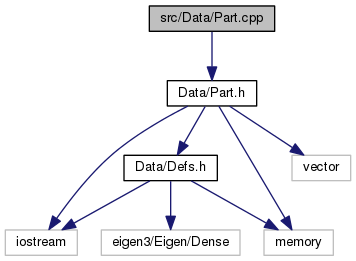
\includegraphics[width=339pt]{_part_8cpp__incl}
\end{center}
\end{figure}

\hypertarget{_vocabulary_8cpp}{\section{src/\-Data/\-Vocabulary.cpp File Reference}
\label{_vocabulary_8cpp}\index{src/\-Data/\-Vocabulary.\-cpp@{src/\-Data/\-Vocabulary.\-cpp}}
}
{\ttfamily \#include \char`\"{}Data/\-Vocabulary.\-h\char`\"{}}\\*
Include dependency graph for Vocabulary.\-cpp\-:\nopagebreak
\begin{figure}[H]
\begin{center}
\leavevmode
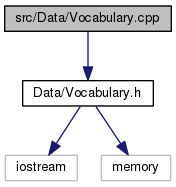
\includegraphics[width=204pt]{_vocabulary_8cpp__incl}
\end{center}
\end{figure}

\hypertarget{_reader_8cpp}{\section{src/\-Utilities/\-Reader.cpp File Reference}
\label{_reader_8cpp}\index{src/\-Utilities/\-Reader.\-cpp@{src/\-Utilities/\-Reader.\-cpp}}
}
{\ttfamily \#include \char`\"{}Utilities/\-Reader.\-h\char`\"{}}\\*
Include dependency graph for Reader.\-cpp\-:\nopagebreak
\begin{figure}[H]
\begin{center}
\leavevmode
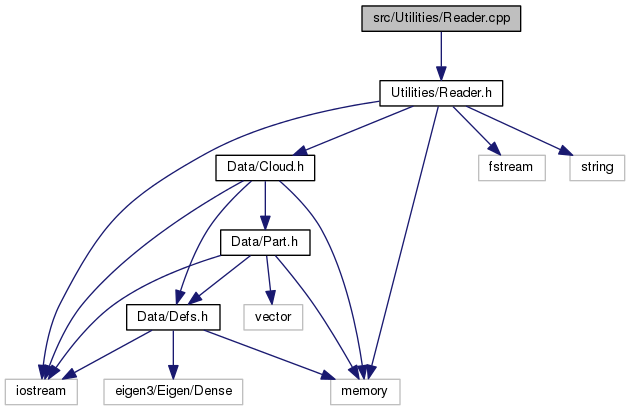
\includegraphics[width=350pt]{_reader_8cpp__incl}
\end{center}
\end{figure}

\hypertarget{_writer_8cpp}{\section{src/\-Utilities/\-Writer.cpp File Reference}
\label{_writer_8cpp}\index{src/\-Utilities/\-Writer.\-cpp@{src/\-Utilities/\-Writer.\-cpp}}
}
{\ttfamily \#include \char`\"{}Utilities/\-Writer.\-h\char`\"{}}\\*
Include dependency graph for Writer.\-cpp\-:\nopagebreak
\begin{figure}[H]
\begin{center}
\leavevmode
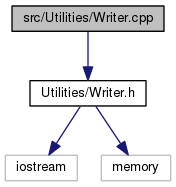
\includegraphics[width=204pt]{_writer_8cpp__incl}
\end{center}
\end{figure}

%--- End generated contents ---

% Index
\newpage
\phantomsection
\addcontentsline{toc}{chapter}{Index}
\printindex

\end{document}
